\documentclass[12pt, spanish]{article}
\usepackage[spanish]{babel}
\selectlanguage{spanish}
%\usepackage{natbib}
\usepackage{url}
\usepackage[utf8x]{inputenc}
\usepackage{graphicx}
\graphicspath{{images/}}
\usepackage{parskip}
\usepackage{fancyhdr}
\usepackage{vmargin}
\usepackage{multirow}
\usepackage{float}
\usepackage{chngpage}

\usepackage{amsfonts}

\usepackage{subcaption}

\usepackage{hyperref}
\usepackage[
    type={CC},
    modifier={by-nc-sa},
    version={4.0},
]{doclicense}

\hypersetup{
    colorlinks=true,
    linkcolor=blue,
    filecolor=magenta,
    urlcolor=cyan,
}

% para codigo
\usepackage{listings}
\usepackage{xcolor}



%% configuración de listings

\definecolor{listing-background}{HTML}{F7F7F7}
\definecolor{listing-rule}{HTML}{B3B2B3}
\definecolor{listing-numbers}{HTML}{B3B2B3}
\definecolor{listing-text-color}{HTML}{000000}
\definecolor{listing-keyword}{HTML}{435489}
\definecolor{listing-identifier}{HTML}{435489}
\definecolor{listing-string}{HTML}{00999A}
\definecolor{listing-comment}{HTML}{8E8E8E}
\definecolor{listing-javadoc-comment}{HTML}{006CA9}

\lstdefinestyle{eisvogel_listing_style}{
  language         = python,
%$if(listings-disable-line-numbers)$
%  xleftmargin      = 0.6em,
%  framexleftmargin = 0.4em,
%$else$
  numbers          = left,
  xleftmargin      = 0em,
 framexleftmargin = 0em,
%$endif$
  backgroundcolor  = \color{listing-background},
  basicstyle       = \color{listing-text-color}\small\ttfamily{}\linespread{1.15}, % print whole listing small
  breaklines       = true,
  frame            = single,
  framesep         = 0.19em,
  rulecolor        = \color{listing-rule},
  frameround       = ffff,
  tabsize          = 4,
  numberstyle      = \color{listing-numbers},
  aboveskip        = 1.0em,
  belowskip        = 0.1em,
  abovecaptionskip = 0em,
  belowcaptionskip = 1.0em,
  keywordstyle     = \color{listing-keyword}\bfseries,
  classoffset      = 0,
  sensitive        = true,
  identifierstyle  = \color{listing-identifier},
  commentstyle     = \color{listing-comment},
  morecomment      = [s][\color{listing-javadoc-comment}]{/**}{*/},
  stringstyle      = \color{listing-string},
  showstringspaces = false,
  escapeinside     = {/*@}{@*/}, % Allow LaTeX inside these special comments
  literate         =
  {á}{{\'a}}1 {é}{{\'e}}1 {í}{{\'i}}1 {ó}{{\'o}}1 {ú}{{\'u}}1
  {Á}{{\'A}}1 {É}{{\'E}}1 {Í}{{\'I}}1 {Ó}{{\'O}}1 {Ú}{{\'U}}1
  {à}{{\`a}}1 {è}{{\'e}}1 {ì}{{\`i}}1 {ò}{{\`o}}1 {ù}{{\`u}}1
  {À}{{\`A}}1 {È}{{\'E}}1 {Ì}{{\`I}}1 {Ò}{{\`O}}1 {Ù}{{\`U}}1
  {ä}{{\"a}}1 {ë}{{\"e}}1 {ï}{{\"i}}1 {ö}{{\"o}}1 {ü}{{\"u}}1
  {Ä}{{\"A}}1 {Ë}{{\"E}}1 {Ï}{{\"I}}1 {Ö}{{\"O}}1 {Ü}{{\"U}}1
  {â}{{\^a}}1 {ê}{{\^e}}1 {î}{{\^i}}1 {ô}{{\^o}}1 {û}{{\^u}}1
  {Â}{{\^A}}1 {Ê}{{\^E}}1 {Î}{{\^I}}1 {Ô}{{\^O}}1 {Û}{{\^U}}1
  {œ}{{\oe}}1 {Œ}{{\OE}}1 {æ}{{\ae}}1 {Æ}{{\AE}}1 {ß}{{\ss}}1
  {ç}{{\c c}}1 {Ç}{{\c C}}1 {ø}{{\o}}1 {å}{{\r a}}1 {Å}{{\r A}}1
  {€}{{\EUR}}1 {£}{{\pounds}}1 {«}{{\guillemotleft}}1
  {»}{{\guillemotright}}1 {ñ}{{\~n}}1 {Ñ}{{\~N}}1 {¿}{{?`}}1
  {…}{{\ldots}}1 {≥}{{>=}}1 {≤}{{<=}}1 {„}{{\glqq}}1 {“}{{\grqq}}1
  {”}{{''}}1
}
\lstset{style=eisvogel_listing_style}


\usepackage[default]{sourcesanspro}

\setmarginsrb{2 cm}{1 cm}{2 cm}{2 cm}{1 cm}{1.5 cm}{1 cm}{1.5 cm}

\title{Práctica 3:\\
Detección de puntos relevantes y creación de panoramas.\hspace{0.05cm} }
\author{Antonio David Villegas Yeguas}
\date{\today}

\renewcommand*\contentsname{hola}

\makeatletter
\let\thetitle\@title
\let\theauthor\@author
\let\thedate\@date
\makeatother

\pagestyle{fancy}
\fancyhf{}
\rhead{\theauthor}
\lhead{\thetitle}
\cfoot{\thepage}

\begin{document}

%%%%%%%%%%%%%%%%%%%%%%%%%%%%%%%%%%%%%%%%%%%%%%%%%%%%%%%%%%%%%%%%%%%%%%%%%%%%%%%%%%%%%%%%%

\begin{titlepage}
    \centering
    \vspace*{0.3 cm}
    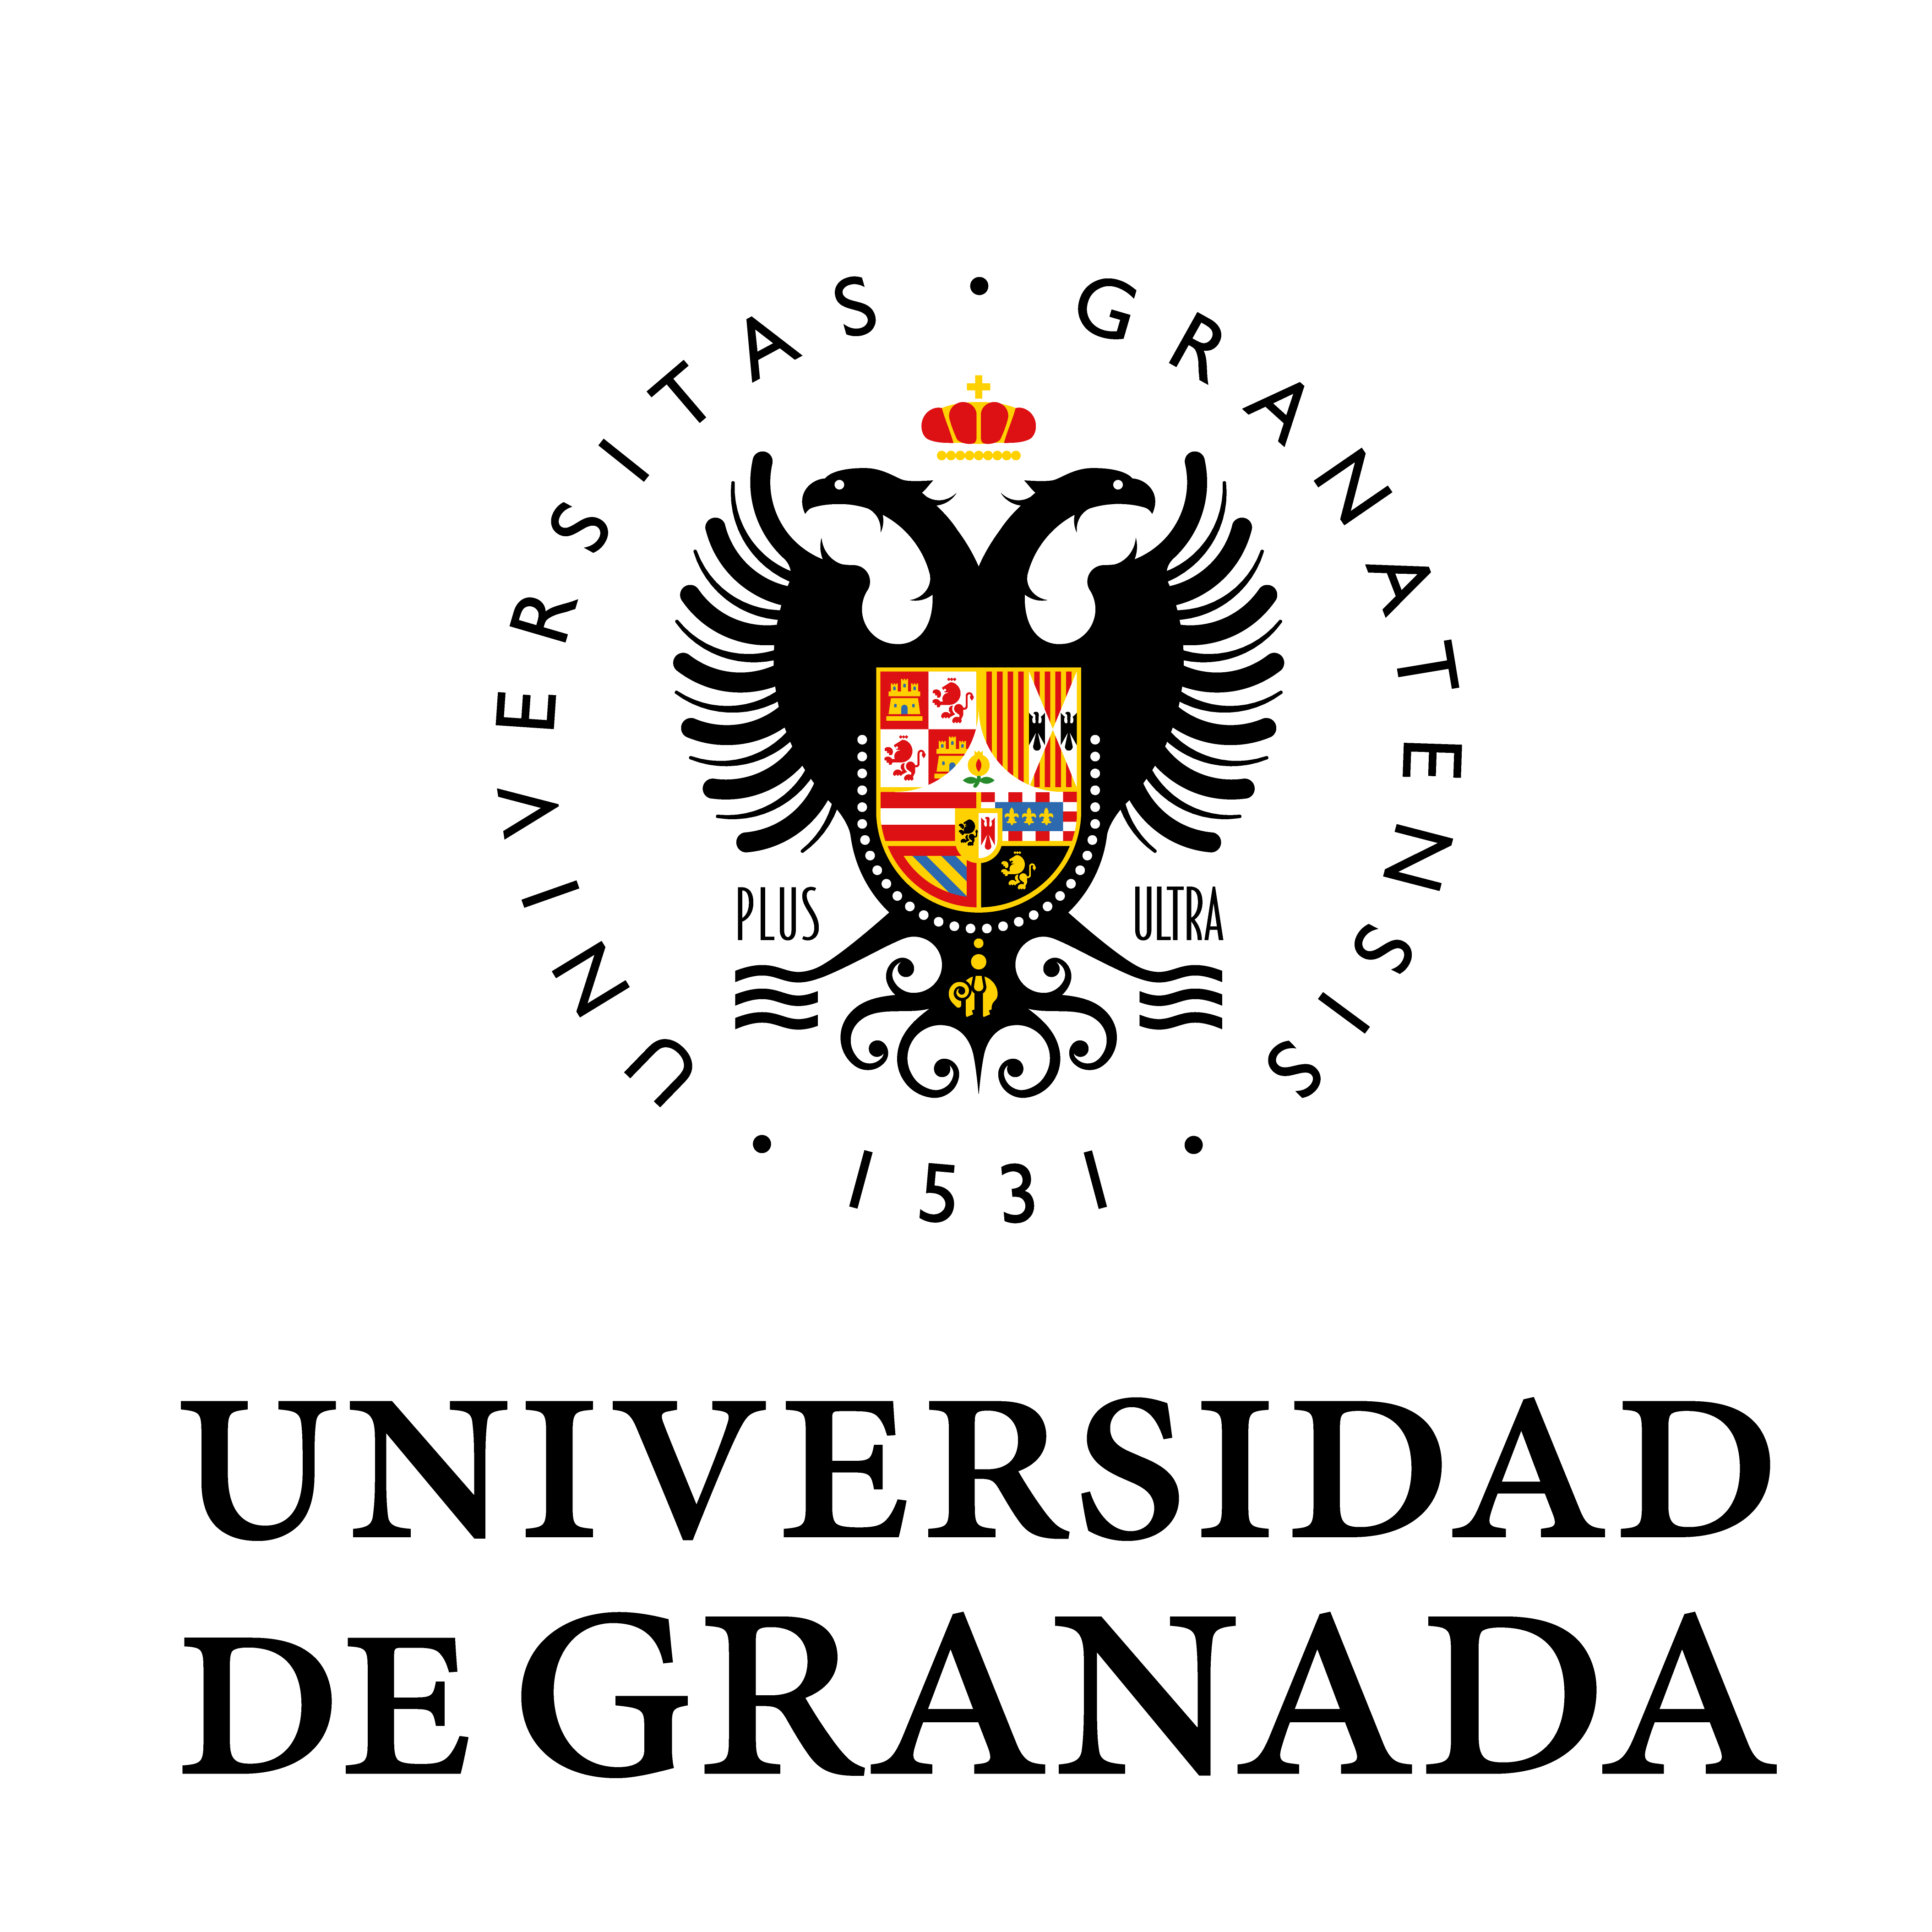
\includegraphics[scale = 0.50]{ugr.png}\\[0.7 cm]
    %\textsc{\LARGE Universidad de Granada}\\[2.0 cm]
    \textsc{\large 4º CSI 2020/21 - Grupo 2}\\[0.5 cm]
    \textsc{\large Grado en Ingeniería Informática}\\[0.5 cm]
    \rule{\linewidth}{0.2 mm} \\[0.2 cm]
    { \huge \bfseries \thetitle}\\
    \rule{\linewidth}{0.2 mm} \\[1 cm]

    \begin{minipage}{0.4\textwidth}
        \begin{flushleft} \large
            \emph{Autor:}\\
            \theauthor\\
			 \emph{DNI:}\\
            77021623-M
            \end{flushleft}
            \end{minipage}~
            \begin{minipage}{0.4\textwidth}
            \begin{flushright} \large
            \emph{Asignatura: \\
            Visión por Computador}   \\
            \emph{Correo:}\\
            advy99@correo.ugr.es
        \end{flushright}
    \end{minipage}\\[0.5cm]

    {\large \thedate}\\[0.5cm]
    %{\url{https://github.com/advy99/VC/}}
    {\doclicenseThis}

    \vfill

\end{titlepage}

%%%%%%%%%%%%%%%%%%%%%%%%%%%%%%%%%%%%%%%%%%%%%%%%%%%%%%%%%%%%%%%%%%%%%%%%%%%%%%%%%%%%%%%%%

\tableofcontents
\pagebreak

%%%%%%%%%%%%%%%%%%%%%%%%%%%%%%%%%%%%%%%%%%%%%%%%%%%%%%%%%%%%%%%%%%%%%%%%%%%%%%%%%%%%%%%%%


\section*{Introducción}

Tras haber realizado una introducción a OpenCV en la práctica cero, trabajado con filtros sobre imágenes en la práctica uno, y clasificado imágenes utilizando redes neuronales convolucionales en la práctica dos, en esta práctica trabajaremos con la información de la geometría de las imágenes, en concreto con la detección de puntos de interes, su detección y uso para realizar otras operaciones como la detección de un objeto o zona de una imagen dentro de otra, lo que también nos permitirá por último crear panoramas de imágenes.

Trabajaremos con puntos Harris, descriptores de puntos con AKAZE, y por último creación de panoramas utilizando los puntos de interes y descriptores AKAZE.

\section{Detección de punto Harris}

Este apartado trata sobre la detección de puntos de interes utilizando el algoritmo de detección de esquinas Harris, que se trata de, utilizando una pirámide gaussiana de la imagen sobre la que obtener los puntos de interes de cara a trabajar con varias escalas y una pirámide con las derivadas de cara a obtener el gradiente, calcular los puntos de interes usando el criterio de Harris, aplicar una supresión de no máximos de cara a quedarse con los más prometedores y con estos calcular su orientación utilizando su gradiente\cite{harris}.

En mayor detalle, para cada escala (nivel de la pirámide construida), realizaremos:

\begin{enumerate}
	\item Detección de puntos de interes: Utilizando la función de OpenCV \texttt{cornerEigenValsAndVecs} obtendremos los valores singulares, para despues aplicarles el criterio Harris: $\frac{\lambda_{1} \lambda_{2}}{\lambda_{1} + \lambda_{2}}$.
	\item Aplicar el umbral Harris: Eliminar los valores por debajo de este umbral.
	\item Supresión de no máximos: Dado un tamaño de ventana, recorreremos la imagen actual con ese tamaño de ventana, obteniendo el valor máximo de la ventana actual, y si el centro de la ventana (pixel actual) es el máximo, almacenaremos ese valor en el resultado, si no, lo descartaremos.
	\item Estimación de la escala de los puntos en píxeles: Como nos dice en el guión, haremos una estimación de la escala de forma que sea igual a $2^{nivel\_piramide - 1} \cdot tam\_bloque$.
	\item Calculo de la orientación de los puntos: Utilizando el gradiente de los puntos considerados de interes, calcularemos la norma de dichos puntos y con eso su orientación. Como nos dice el guión, en este apartado utilizaremos el gradiente de las imágenes aplicandole un alisamiento con $\sigma = 4.5$.
	\item Calculo del KeyPoint de OpenCV utilizando el método \texttt{KeyPoint} y los valores calculados.
\end{enumerate}

Y con esto ya tendremos los puntos de interes. Además de estos puntos, la función implementada devolverá los puntos corregidos, que son calculados de la siguiente forma:

\begin{enumerate}
	\item Concatenar los valores de X e Y de los puntos en un vector fila, de cara a poder utilizarlos en el siguiente punto.
	\item Utilizar el método \texttt{cornerSubPix} como nos dice el guión para obtener los puntos corregidos, usando como criterio de parada quince iteraciones o un epsilon menos a $0.01$. Se han escogido estos valores ya que han funcionado bastante bien de forma empírica.
	\item Redondeo y adaptación de los ejes de los puntos obtenidos por la función \texttt{cornerSubPix}.
\end{enumerate}


Como vemos, en este apartado tenemos bastantes parámetros con los que trabajar:

\begin{enumerate}
	\item Tamaño del bloque: Fijado a cinco, como nos decía el guión, podía ser desde 3x3 a 7x7, en mi caso el tamaño cinco se ha comportado bastante bien de forma empírica, y por eso lo he escogido.
	\item Tamaño de la ventana: En este caso se nos daba entre utilizar tamaños 3x3, 5x5 y 7x7. Al utilizar tamaños más pequeños se obtenian muchos más puntos, ya que tendríamos un mayor número de ventanas, pero se obtenian demasiados puntos para el umbral utilizado (que comentaré más adelante), por este motivo he utilizado el tamaño 7x7.
	\item Número de escalas: Como nos decía el guión, tres escalas.
	\item Sigma de la pirámide Gaussiana: En este caso, como nos comentaba el guión, he utilizado $\sigma = 4.5$.
	\item Umbral del criterio Harris: Como nos decía la bibliografía\cite{harris}, he utilizado un umbral $t = 10.0$, en los resultados de este apartado pondré un ejemplo de utilizar un umbrál distinto.
	\item Tamaño del kernel para calcular las derivadas: En este caso también se nos recomendaban los valores de ksize de tres o cinco, y en mi caso he optado por el valor tres ya que se comportaba de forma correcta.
\end{enumerate}

Tras describir la función con la que obtenemos los puntos Harris a las distintas escalas, para visualizarlos simplemente se ha usado una lista con todos los puntos (de todas las escalas), y se ha utilizado el método \texttt{drawKeypoints} para dibujarlos sobre la imagen, utilizando la opción\\  \texttt{DRAW\_MATCHES\_FLAGS\_DRAW\_RICH\_KEYPOINTS} de forma que dibujará los puntos acorde a la escala, y con su orientación.

Otro detalle a tener en cuenta es que aunque se ha utilizado la imagen en blanco y negro para obtener los puntos (como nos recomendaba el guión y nos obliga OpenCV), se han mostrado sobre la imagen a color para quela distinción de los puntos sobre la imagen sea más llamativa. Se ha obtenido el siguiente resultado:


\begin{figure}[H]
  \centering
      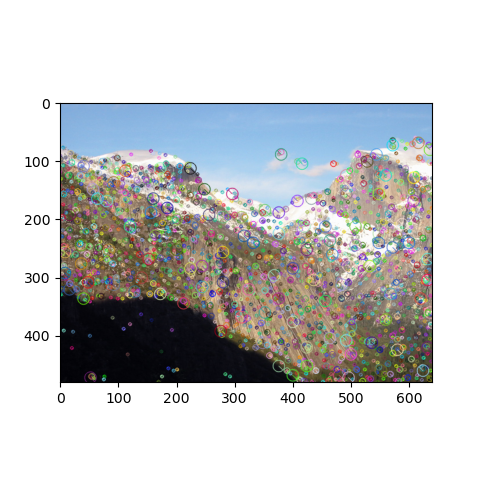
\includegraphics[width=\textwidth]{p_harris_h_10.png}
 		\caption{Puntos Harris sobre la imágen Yosemite1.}
\end{figure}

\begin{figure}[H]
  \centering
      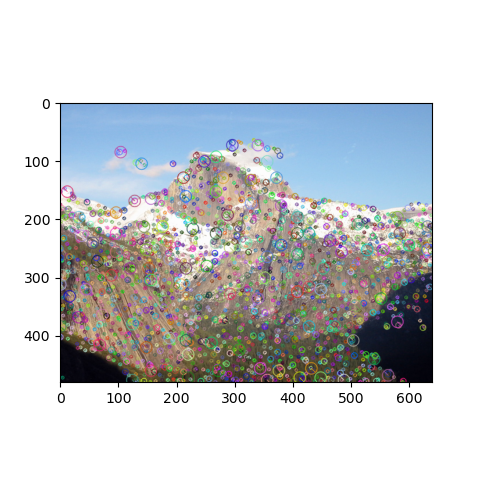
\includegraphics[width=\textwidth]{p_harris_h_10_y2.png}
 		\caption{Puntos Harris sobre la imágen Yosemite2.}
\end{figure}

Como vemos los resultados son bastante buenos, y como se nos pedía, hemos calculado unos 2000 puntos en cada imágen, distribuidos de la siguiente forma.

Para la imagen Yosemite1:

\begin{lstlisting}
La escala  0  tiene  1478  puntos
La escala  1  tiene  375  puntos
La escala  2  tiene  109  puntos
\end{lstlisting}

Para la imagen Yosemite2:

\begin{lstlisting}
La escala  0  tiene  1506  puntos
La escala  1  tiene  392  puntos
La escala  2  tiene  114  puntos
\end{lstlisting}

Tal y como nos pedía el guión, alrededor de un 70\% de los puntos en el nivel más grande, un 25\% en el siguiente nivel, y por último el 5\% restante en el nivel más bajo.


Como hemos visto, la mayoría de parámetros son parámetros que ya hemos visto y estudiado en otras prácticas (en especial la primera), sin embargo, aquí aparece un nuevo parámetro, el umbral Harris, que de cara a estudiar su importancia, he repetido la prueba de Yosemite1 pero utilizando un umbral de 300 en lugar de 10:

\begin{figure}[H]
  \centering
      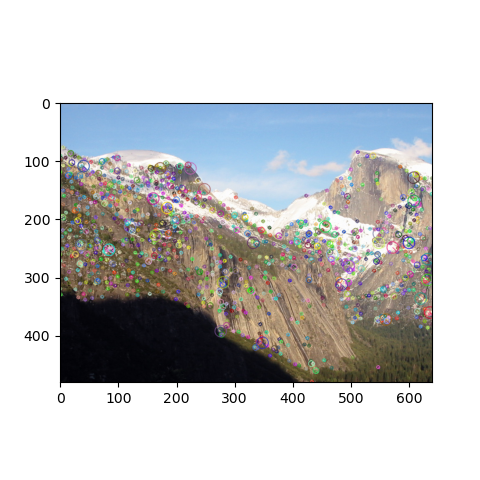
\includegraphics[width=\textwidth]{p_harris_h_300.png}
 		\caption{Puntos Harris sobre la imágen Yosemite1 con umbral Harris de 300.}
\end{figure}

Con el que obtenemos el siguiente número de puntos:

\begin{lstlisting}
La escala  0  tiene  915  puntos
La escala  1  tiene  155  puntos
La escala  2  tiene  31  puntos
\end{lstlisting}

Como era de esperar, se eliminan muchos de los puntos de interes obtenidos, aunque los parámetros son los mismos a excepción del umbral, por lo que este parámetro nos puede ayudar a ajustar el número de puntos a obtener manteniendo la forma de calcular los distintos puntos, al mantener los tamaños de bloque, ksize, entre otros.



Por último para este ejercicio compararemos los puntos originales con los puntos corregidos.

Para realizar esta comparación se han escogido tres puntos al azar donde su posición original es distinta a la posición corregida, y se han dibujado como círculos de radio 2 píxeles en la imagen, para despues mostrar una ventana de 9x9 como nos piden, de forma que se distinga la posición de los puntos. El resultado es el siguiente, con el punto original en azul y en rojo el corregido:

\begin{figure}[H]
  \centering
      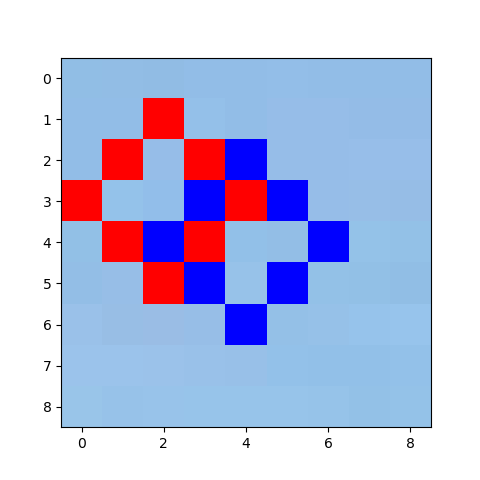
\includegraphics[width=\textwidth]{cmp_p1.png}
 		\caption{Primer punto corregido escogido al azar.}
\end{figure}

\begin{figure}[H]
  \centering
      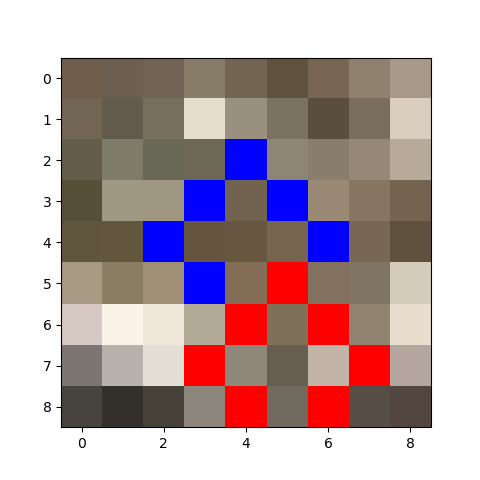
\includegraphics[width=\textwidth]{cmp_p2.png}
 		\caption{Segundo punto corregido escogido al azar.}
\end{figure}

\begin{figure}[H]
  \centering
      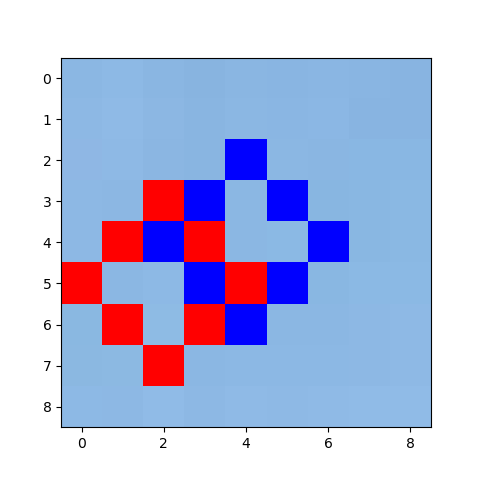
\includegraphics[width=\textwidth]{cmp_p3.png}
 		\caption{Tercer punto corregido escogido al azar.}
\end{figure}


Se puede observar como se modifican ligeramente las posiciones de los puntos, y a excepción del tercer punto donde todo el fondo es azul claro, en los otros dos casos se mmueve a una zona donde hay una mayor variación entre píxeles.


\section{Descriptores AKAZE y correspondencias entre dos imágenes}

En este apartado nos centraremos en dectecar los puntos de interes así como sus descriptores utilizando AKAZE\cite{akaze}, la versión acelerada de KAZE\cite{kaze}.

Para este ejercicio

\section{Mosaico de imágenes}

\section{Mosaico con multiples imágenes}



\newpage

\section{Referencias, material y documentación usada}


\begin{thebibliography}{9}

	\bibitem{harris}

		Multi-Image Matching using Multi-Scale Oriented Patches --- Matthew Brown, Richard Szeliski y Simon Winder

		\url{http://matthewalunbrown.com/papers/cvpr05.pdf}

	\bibitem{kaze}

		KAZE Features --- Pablo F. Alcantarilla, Adrien Bartoli, and Andrew J. Davison (Enlace de The Wayback Machine ya que el enlace original no funciona).

		\url{https://web.archive.org/web/20200125092345/http://www.robesafe.com/personal/pablo.alcantarilla/papers/Alcantarilla12eccv.pdf}

	\bibitem{akaze}

		Fast Explicit Diffusion for AcceleratedFeatures in Nonlinear Scale Spaces --- Pablo F. Alcantarilla, Jesús Nuevo and Adrien Bartoli (Enlace de The Wayback Machine ya que el enlace original no funciona).

		\url{https://web.archive.org/web/20200114013631/http://www.robesafe.com/personal/pablo.alcantarilla/papers/Alcantarilla13bmvc.pdf}



\end{thebibliography}

\end{document}
